\section{Evaluation results}
Subsection \ref{subsec:per_mes} contains the regular performance evaluation measures, such as recall, precision and F-measure. The example in subsection \ref{subsec:eval_example} will clarify how the performance measures have been obtained. The type prediction distribution in subsection \ref{subsec:type_pred} shows the varying difficulty in predicting specific types.

\label{sec:eva}
\subsection{Performance measures}\label{subsec:per_mes}
The performance evaluation for the different test sets can be seen in figure \ref{fig:performance}. The CoNLL performance is an average of both the \textit{ned.testa} -and \textit{ned.testb} set. The parliamentary item set is of the same size as ned.testa. The last column in the figure shows performance after reclassification (\ref{subsec:reclas}) of entity types in the parliamentary items set. For all measures evaluation is done \textbf{per token}. Accuracy is obtained by binarily evaluating all tokens: if a token is predicted as an NE (regardless of type), but it turns out not to be, this token prediction is marked as incorrect. Tokens not seen as an entity while they are, idem. Low accuracy would be the result of Frog incorrectly identifying non-entities as entities, since the other way around would not hit accuracy hard due to the sparcity of entities in both test sets. Recall is measured as the proportion of retrieved tokens tagged as an entity that were annotated in the test set, again not looking at entity type. IOB precision is the precision of the first part of the entity tag (figure \ref{fig:iob}). This will measure how precisely the beginning of an entity consisting of multiple tokens has been found, or how succesfully different entities following each other have been seperated. Type precision is decided on the second part of the entity tag.  Regular precision is the combination of type precision en IOB precision. F-measure is the harmonic mean of the regular precision and the recall.

\subsection{Evaluation example}\label{subsec:eval_example}
To examplify the performance measures, a single sentence has been evaluated in figure \ref{fig:eval_example}. The accuracy is $\frac{9}{10}$, because \textit{S.A.M.} was not predicted as an entity. This miss is also noticeable in recall, to which a score of $\frac{4}{5}$ is assigned. Type -and IOB precision are only calculated for the recalled entities. Assigning the wrong type to \textit{Kabeljauwherstelplan} makes for a type precision of $\frac{3}{4}$. Recognizing \textit{Dijksma} as the first instead of the second token of the person entity determines the IOB precision at $\frac{3}{4}$. The last column shows the evaluation for the regular precision, which is $\frac{2}{4}$, as both type and IOB need to be correct.

\begin{figure}
\begin{center}
\begin{tabular}{l||r|r|r|}
     & \multicolumn{1}{l|}{\textbf{CoNLL}} & \multicolumn{1}{l|}{\textbf{Parliamentary items}} & \multicolumn{1}{m{4cm}|}{\textbf{Parliamentary items + reclassification}} \\\hline \hline
Accuracy & 0.950 & 0.973 & 0.974 \\\hline
Recall & 0.845 & 0.906 & 0.908\\\hline 
IOB precision & 0.915 & 0.890 & 0.890 \\\hline 
Type precision & 0.672 & 0.616 & 0.662\\\hline 
Precision & 0.629 & 0.563 & 0.603\\\hline
F-measure & 0.720 & 0.694 & 0.725\\\hline
 \end{tabular}
\caption{Performance overview of both sets}
\label{fig:performance}
\end{center}
\end{figure}

\begin{figure}
\begin{center}
\begin{tabular}{|l||l|l|l|l|l|l|l|}
\multicolumn{6}{l}{\large{S.A.M. Dijksma vergaderde over het Kabeljauwherstelplan in Ter Heijde.}} \\\hline
\multicolumn{1}{|l|}{\textbf{Token}} & \multicolumn{1}{l|}{\textbf{Predicted}} & \multicolumn{1}{l|}{\textbf{Correct}} & \textbf{Recalled} & \textbf{Type} & \textbf{IOB} & \textbf{Precise} \\\hline \hline
S.A.M. & O & B-PER & $\times$ & N/A & N/A & N/A \\\hline 
Dijksma & B-PER & I-PER & $\checked$ & $\checked$ & $\times$ & $\times$\\\hline 
vergaderde & O & O & N/A & N/A & N/A & N/A\\\hline 
over & O & O & N/A & N/A & N/A & N/A\\\hline  
het & O & O & N/A & N/A & N/A & N/A\\\hline 
Kabeljauwherstelplan & B-ORG & B-MISC & $\checked$ & $\times$ & $\checked$ & $\times$\\\hline 
in & O & O & N/A & N/A & N/A & N/A\\\hline 
Ter & B-LOC & B-LOC & $\checked$ & $\checked$ & $\checked$ & $\checked$\\\hline 
Heijde & I-LOC & I-LOC & $\checked$ & $\checked$ & $\checked$ & $\checked$\\\hline 
. & O & O & N/A & N/A & N/A & N/A\\\hline
\end{tabular}
\caption{Evaluation example}
\label{fig:eval_example}
\end{center}
\end{figure}

\subsection{Type prediction}\label{subsec:type_pred}
Since type precision has appeared to be relatively low, it would be interesting to analyze errors made per type. Figure \ref{fig:confusion} shows a prediction distribution for each type. 
It can be seen that location as a type is predicted very accurately, while prediction of the type person seems to be significantly more difficult. A plausible explanation for this could be the effectiveness of gazetteers per type. Location names such as \textit{Den Haag}, \textit{Amsterdam} and \textit{Nederland} appear very frequent in parliamentary items and are more easily covered by a plain gazetteer, while person names are incredibly hard to cover in the same way. Ambiguity is, inter alia, caused by abbreviations. Aditionally, locations are almost never written shorthand. Organizations, however, especially political organs, often appear in shortened form. 

\begin{figure}[h]
    \centering
    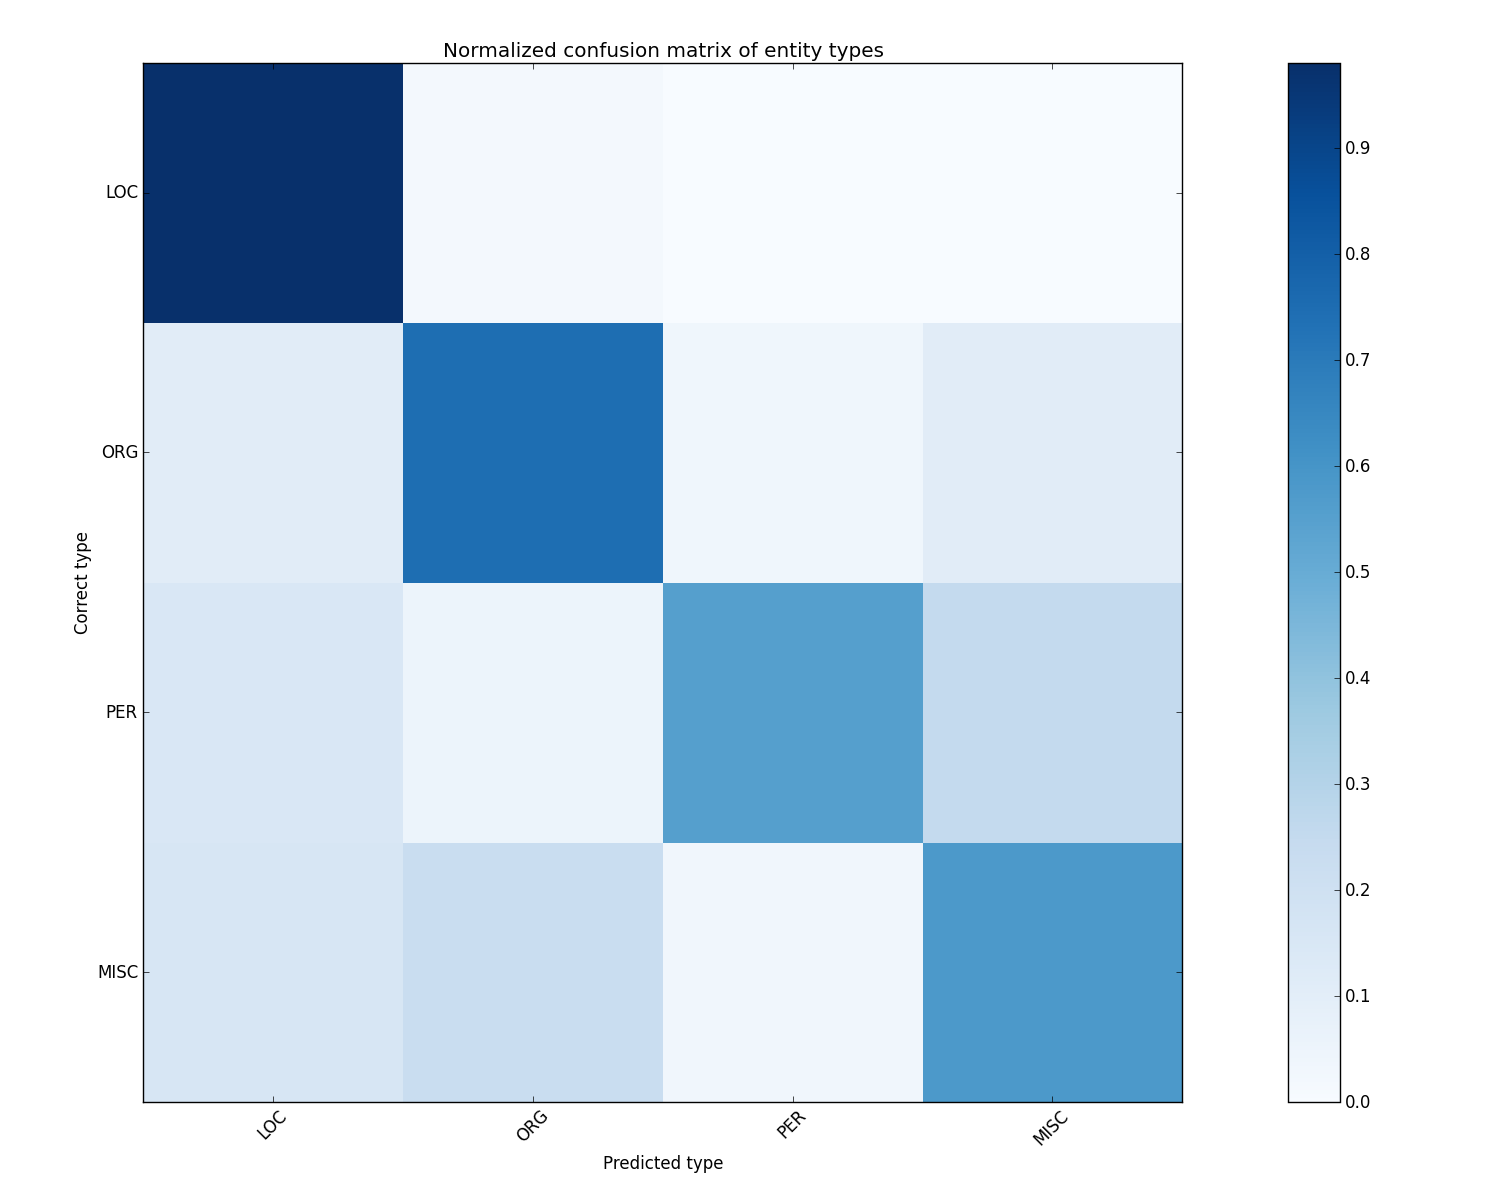
\includegraphics[scale=0.4]{fig/confusion_matrix_reclassified}
    \caption{Prediction distribution per type}
    \label{fig:confusion}
\end{figure}
